\section{Exponential Functions, Logarithms and e}

\begin{frame}{Bacterial Growth on the Human Body}
  \begin{itemize}
    \item Our skin (and other areas like the mouth, nose, and intestines) hosts hundreds of thousands of microscopic organisms.
    \item In fact, bacterial cells in our body outnumber our own cells.
    \item While some bacteria can cause illness, many are essential for our health.
    \item Bacteria reproduce through binary fission—each cell splits into two.
    \item Under ideal conditions, a single bacterium doubling every hour can lead to over 1,000 cells in 10 hours and more than 16 million in 24 hours.
  \end{itemize}
\end{frame}

\begin{frame}{Bacterial Growth Over Time}
  \begin{table}[ht]
    \centering
    \begin{tabular}{c|ccccccccccc}
      \textbf{Hour} & 0 & 1 & 2 & 3 & 4 & 5 & 6 & 7 & 8 & 9 & 10 \\ \hline
      \textbf{Bacteria} & 1 & 2 & 4 & 8 & 16 & 32 & 64 & 128 & 256 & 512 & 1024 \\
    \end{tabular}
    \caption{Bacterial cell count doubling every hour.}
  \end{table}
\end{frame}

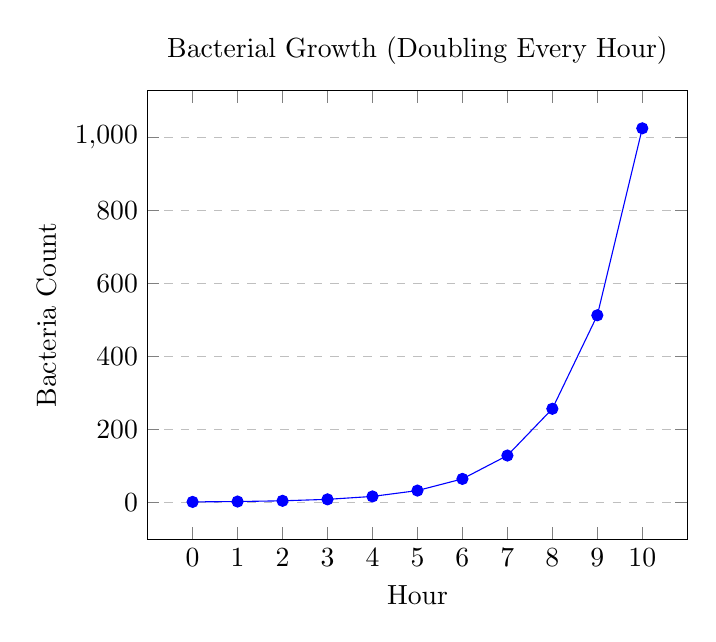
\begin{tikzpicture}
  \begin{axis}[
      xlabel={Hour},
      ylabel={Bacteria Count},
      title={Bacterial Growth (Doubling Every Hour)},
      xtick={0,1,2,3,4,5,6,7,8,9,10},
      ymajorgrids=true,
      grid style=dashed,
      % Uncomment the following line for a logarithmic scale on the y-axis:
      % ymode=log,
    ]
    \addplot[
      color=blue,
      mark=*,
      ]
      coordinates {
        (0,1) (1,2) (2,4) (3,8) (4,16) (5,32) (6,64) (7,128) (8,256) (9,512) (10,1024)
      };
  \end{axis}
\end{tikzpicture}

\begin{frame}{Population Growth in India}
  \begin{itemize}
    \item India is the second most populous country, with about 1.39 billion people in 2021.
    \item Its population grows at an annual rate of roughly 1.2\%.
    \item If this trend continues, India's population is projected to exceed China’s by 2027.
    \item While rapid population increases are often described as "exponential," in mathematics the term has a very precise meaning.
  \end{itemize}
\end{frame}

\begin{frame}{Defining Exponential Growth}
  \begin{block}{Key Concepts}
    \begin{itemize}
      \item \textbf{Percentage Change:} 
      \begin{itemize}
        \item refers to a change based on a percent of the original amount
      \end{itemize}
      \item \textbf{Exponential Growth:} 
        \begin{itemize}
          \item refers to an increase based on a constant multiplicative rate of change over equal increments of time, that is, a percent increase of the original amount over time.
          \item For example, if a quantity doubles each period, that is a 100\% increase per period.
        \end{itemize}
      \item \textbf{Linear Growth:} 
        \begin{itemize}
          \item The original value increases by a fixed \textbf{amount} (additive rate) over equal time intervals.
        \end{itemize}
        \item \textbf{Exponent Decay:}
        \begin{itemize}
          \item refers to a decrease based on a constant multiplicative rate of change over equal increments of time, that is, a percent decrease of the original amount over time.
        \end{itemize}
    \end{itemize}
  \end{block}
\end{frame}

\begin{frame}{Exponential Function and Its Behavior}
  \begin{block}{Definition}
    Suppose \(b>0\) with \(b\neq 1\). Then the \emph{exponential function} with base \(b\) is defined by
    \[
      f(x)=b^x.
    \]
    For example, if \(b=2\), then \(f(x)=2^x\). (Note that \(2^x\) is different from \(x^2\).)
  \end{block}
  \vspace{0.5em}
  \begin{block}{Behavior (for \(b>1\))}
    \begin{itemize}
      \item \textbf{Domain:} All real numbers, \(\mathbb{R}\).
      \item \textbf{Range:} All positive numbers, \((0,\infty)\).
      \item \(f(x)=b^x\) is an \emph{increasing} function.
      \item \(b^x\) becomes very large as \(x\) increases.
      \item \(b^x\) approaches \(0\) as \(x\) becomes very negative.
    \end{itemize}
  \end{block}
\end{frame}

\begin{frame}{Comparing Exponential and Linear Growth}
  \begin{table}[ht]
    \centering
    \begin{tabular}{c|c|c}
      \(x\) & \(f(x)=2^x\) & \(g(x)=2x\) \\ \hline
      0 & 1 & 0 \\
      1 & 2 & 2 \\
      2 & 4 & 4 \\
      3 & 8 & 6 \\
      4 & 16 & 8 \\
      5 & 32 & 10 \\
      6 & 64 & 12 \\
    \end{tabular}
    \caption{Exponential vs. Linear Growth.}
  \end{table}
\end{frame}


\begin{frame}{Example: The Function \(f(x)=2^x\)}
  \begin{block}{Exponential Growth Illustrated (Table 2)}
    \begin{table}[ht]
      \centering
      \begin{tabular}{|c|c|c|c|c|c|c|c|}
        \hline
        \(x\)      & -3 & -2 & -1 & 0 & 1 & 2 & 3 \\ \hline
        \(2^x\) & \(2^{-3}=\frac{1}{8}\) & \(2^{-2}=\frac{1}{4}\) & \(2^{-1}=\frac{1}{2}\) & \(2^0=1\) & \(2^1=2\) & \(2^2=4\) & \(2^3=8\) \\ \hline
      \end{tabular}
      \caption{Exponential values of \(2^x\) for \(x=-3,\dots,3\).}
    \end{table}
  \end{block}
  \vspace{1em}
  \textbf{Observation:} As \(x\) increases by 1, the output of \(2^x\) doubles, clearly illustrating exponential growth.
\end{frame}




\begin{frame}{Algebraic Properties of Exponents}
  \begin{block}{Properties}
    Let \(a, b > 0\) and \(x, y \in \mathbb{R}\). Then:
    \begin{itemize}
      \item \(b^x \cdot b^y = b^{x+y}\)
      \item \((b^x)^y = b^{xy}\)
      \item \(a^x \cdot b^x = (ab)^x\)
      \item \(b^0 = 1\)
      \item \(b^{-x} = \dfrac{1}{b^x}\)
      \item \(\dfrac{b^x}{b^y} = b^{x-y}\)
      \item \(\dfrac{a^x}{b^x} = \Bigl(\dfrac{a}{b}\Bigr)^x\)
    \end{itemize}
  \end{block}
\end{frame}

\begin{frame}
  \frametitle{Exponent Graph}
  \begin{columns}
    \begin{column}{0.5\textwidth}
      \begin{figure}
        \centering 
        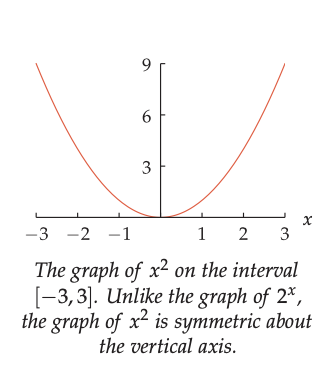
\includegraphics[scale=0.3]{exp-vs-poly1.png}
       \end{figure}      
    \end{column}
 

    \begin{column}{0.5\textwidth}
      \begin{figure}
        \centering 
        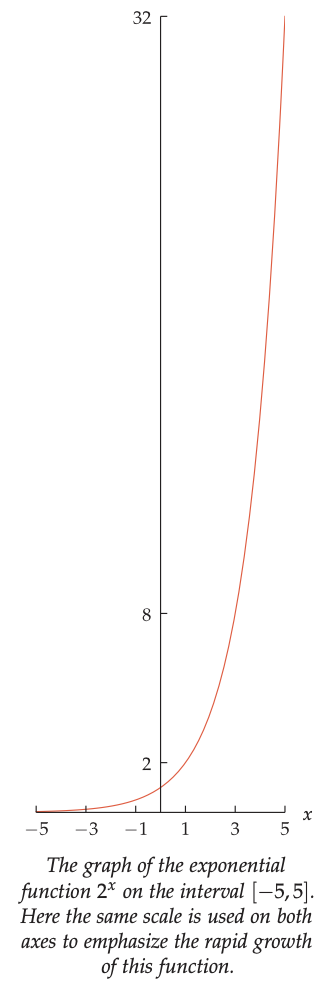
\includegraphics[scale=0.2]{exp-vs-poly2.png}
       \end{figure}      
    \end{column}
  \end{columns}
\end{frame}


  \begin{frame}{Logarithm}
    \begin{block}{Definition}
      Suppose \(b\) and \(y\) are positive numbers with \(b\neq 1\). 
      \begin{itemize}
        \item The logarithm base \(b\) of \(y\), denoted \(\log_b y\), is defined as the unique number \(x\) such that
        \[
          b^x = y.
        \]
        \item  Short Version
        \[
          \log_b y = x \quad \text{means} \quad b^x = y.
        \]
      \end{itemize}
    \end{block}
  \end{frame}

  \begin{frame}{Logarithm of 1 and the Base}
    \begin{block}{Key Properties}
      Let \(b>0\) with \(b\neq 1\). Then:
      \begin{itemize}
        \item \(\log_b 1 = 0\) because \(b^0 = 1\),
        \item \(\log_b b = 1\) because \(b^1 = b\).
      \end{itemize}
    \end{block}
  \end{frame}

  \begin{frame}{Logarithm as an Inverse Function}
    \begin{block}{Definition}
      Suppose \(b\) is a positive number with \(b \neq 1\) and the exponential function \(f\) is defined by
      \[
        f(x) = b^x.
      \]
      Then the inverse function \(f^{-1}\) is given by
      \[
        f^{-1}(y) = \log_b y.
      \]
    \end{block}
  \end{frame}
  
  \begin{frame}{Inverse Properties of Logarithms - Summary}
    \begin{itemize}
      \item \textbf{Inverse Relationship:}
        \begin{itemize}
          \item \(\log_b x\) is the inverse of \(b^x\).
          \item Flipping the graph of \(b^x\) across the line \(y=x\) yields the graph of \(\log_b x\).
        \end{itemize}
      \item \textbf{Monotonicity:}
        \begin{itemize}
          \item For \(b>1\), \(b^x\) is increasing, so \(\log_b x\) is also increasing.
        \end{itemize}
      \item \textbf{Key Equations:}
        \begin{itemize}
          \item \(b^{\log_b y} = y\)
          \item \(\log_b (b^x) = x\)
        \end{itemize}
      \item \textbf{Function-Inverse Properties:}
        \begin{itemize}
          \item These can be written as \((f \circ f^{-1})(y) = y\) and \((f^{-1} \circ f)(x) = x\).
        \end{itemize}
      \item \textbf{Understanding:}
        \begin{itemize}
          \item These properties are fundamental to the relationship between exponential and logarithmic functions.
        \end{itemize}
    \end{itemize}
  \end{frame}

  \begin{frame}{Logarithm of a Power}
    \begin{block}{Property}
      If \(b\) and \(y\) are positive numbers, with \(b \neq 1\), and \(t\) is a real number, then
      \[
        \log_b\left(y^t\right) = t \log_b y.
      \]
    \end{block}
  \end{frame}
\begin{frame}
  \frametitle{Radioactive Decay}
  If a radioactive isotope has half-life \(h\), then the function modeling the number of
  atoms in a sample of this isotope is
  \[ a(t) = a_{0}2^{-t/h}\]
  where \(a_{0}\) is the number of atoms of the isotope in the sample at time \(0\)
  \end{frame} 


  \begin{frame}
  \frametitle{Exponential Growth}
  \begin{block}{A story}
A mathematician in ancient India invented the game of chess. Filled with gratitude for the remarkable entertainment of this game, the king offered themathematician anything he wanted. The king expected the mathematician to
ask for rare jewels or a majestic palace.
But the mathematician asked only that he be given one grain of rice for the
first square on a chessboard, plus two grains of rice for the next square, plus
four grains for the next square, and so on, doubling the amount for each square,
until the 64th square on an 8-by-8 chessboard had been reached. The king was
pleasantly surprised that the mathematician had asked for such a modest reward.
A bag of rice was opened, and first 1 grain was set aside, then 2, then 4, then 8,
and so on. As the eighth square  was
reached, 128 grains of rice were counted out. The king was secretly delighted
to be paying such a small reward and also wondering at the foolishness of the
mathematician.
  \end{block}
  
  \end{frame}

  \begin{frame}
    \begin{block}{Story Cont..}
      As the 16th square was reached, 32,768 grains of rice were counted out—this
was a small part of a bag of rice. But the 21st square required a full bag of rice,
and the 24th square required eight bags of rice. This was more than the king had
expected. However, it was a trivial amount because the royal granary contained
about 200,000 bags of rice to feed the kingdom during the coming winter.
As the 31st square was reached, over a thousand bags of rice were required
and were delivered from the royal granary. Now the king was worried. By the
37th square, the royal granary was two-thirds empty. The 38th square would have
required more bags of rice than were left. The king then stopped the process
and ordered that the mathematician's head be chopped off as a warning about
the greed induced by exponential growth
    \end{block}
  \end{frame}
  \begin{frame}
    \frametitle{Mathematical analysis}
    \begin{itemize}
      \item \(64^{th}\) square requires \( 2^{63} \) grains \(\approx\) \(2^{3}* (2^{10})^{6} = 8*(10^{3})^{6} = 8*10^{18} \approx 10^{19} \) 
      \item if one large bag = \(10^{6} \) grains of rice , then total bags = \(10^{19}/10^{6} \) 
      \item In 2025 India's population is \(\approx 1 * 10^{9} \)
    \end{itemize}
     
    \end{frame}

    \begin{frame}
      \frametitle{Exponential Growth}
      \begin{block}{Definition}
      A function \(f\) is said to have \textbf{exponential growth} if \(f(x) = cb^{kx} \) where 
      \(c\) and \(k\) are positive numbers and \(b > 1\)
      \end{block}
      \begin{itemize}
        \item \(f(x) > p(x)\)  where \(f\) is exponenetial and \(p\) is polynomial for sufficiently large \(x\) 
        \item \(2^{x} > x^{1000} \)  \(\forall \;\; x > 13747 \)  
        \item A function \(f\) has exponential growth if and only if the graph of \(\log f(x)\) is a line with a positive slope
      \end{itemize}


    \end{frame}
    

    \begin{frame}
      \frametitle{Population Growth}
        \begin{block}{Exponential Growth}
          \[
            p(t) = p_0\,e^{rt}
          \]
          \begin{itemize}
            \item \(p_0\): initial population  
            \item \(r\): constant per-capita growth rate  
            \item Assumes unlimited resources → population grows without bound  
            \item Populations of various organisms, ranging from bacteria to humans, often exhibit exponential growth
          \end{itemize}
        \end{block}
    \end{frame}
    \begin{frame}
      \frametitle{Population Growth: Example}
      Suppose a colony of bacteria in a petri dish has 700 cells at 1 pm. These bacteria
      reproduce at a rate that leads to doubling every three hours. How many bacteria
      cells will be in the petri dish at 9 pm on the same day?
      \pause 
      \[
       p(t) = p_{0}2^{t/3} \implies 700 \cdot 2^{8/3} 
       \]
    \end{frame}


    \begin{frame} 
      \frametitle{Population Growth}
      \begin{block}{Exponential growth and doubling}
        If a population doubles every \( d \) time units, then the function \( p \) modeling this population growth is given by the formula

        \[
          p(t) = p_{0} \cdot 2^{(t-t_{0})/d}
        \]
        where \(p_{0}\) is the population at time \(t_{0}\)
        \end{block}    
    \end{frame}

    \begin{frame}
      \frametitle{Compound Interest}
      \begin{figure}
        
\includegraphics[scale=0.2]{CI-comic.png}
      \end{figure}
    \end{frame}

    \begin{frame}
      \frametitle{Example}
      Suppose you deposit \(8000\) in a bank account that pays \(5\%\) annual interest. Assume the bank pays interest once per year at the end of the year, and that each year you place the interest in a cookie jar for safekeeping.
      \begin{enumerate}
        \item  How much will you have (original amount plus interest) at the end of two
        years?
        \item How much will you have (original amount plus interest) at the end of t years?
      \end{enumerate}
      \pause 
      Interest per year \( = 8000*0.05 = 400 \). For 2 years \( = 400*2 = 800\)

      After \(t\) years \(= 8000 + 8000*0.05*t = 8000(1+0.05t)\)
    \end{frame}

    \begin{frame}
      \frametitle{Simple Interest}
      \begin{block}{Simple Interest}
        If interest is paid once per year at the annual rate of \(r\), with no interest paid on the interest, then after \(t\) years 
        an initial amount \(P\) grows to 
        \[
           P(t) = P_{0}(1 + rt) 
        \]
        
      \end{block}
    \end{frame}

    \begin{frame}
      \frametitle{Example}
      Suppose you deposit \(8000\) in a bank account that pays \(5\%\) annual interest. Assume the bank pays interest once per year at the end of the year, and that each year the interest is deposited in the bank account
      \begin{enumerate}
        \item How much will you have at the end of one year?
        \item How much will you have at the end of two years?
        \item How much will you have at the end of t years?
      \end{enumerate}
      \pause 
      \begin{enumerate}
        \item  At the end of an year \( =  8000 + 8000*0.05  = 8400 \implies 8000(1+0.05)\)
        \item  At the end of 2 year \( = 8400 + 8400*0.05 \implies 8400( 1 + 0.05) = 8000(1.05)^{2} \) 
        \item  At the end of \(t\) years \(= 8000(1.05)^{t}\)
      \end{enumerate}
     
    \end{frame}

    \begin{frame}
      \frametitle{SI vs CI}
      \begin{figure}
        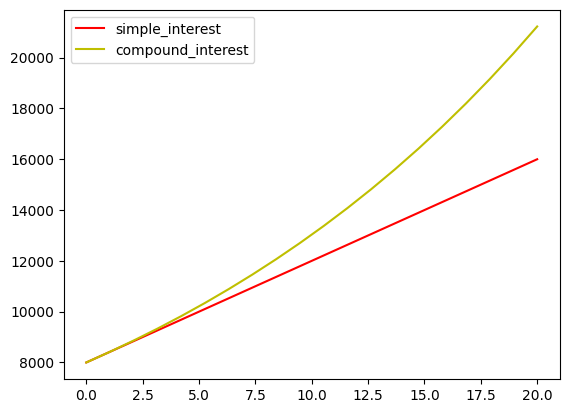
\includegraphics[scale=0.5]{SI_vs_CI.png}
      \end{figure}
    \end{frame}

    \begin{frame}
      \frametitle{Example}
\begin{itemize}
  \item Interest is often compounded more than once per year 
  \item In the above example,if the interest is compunded twice an year means instead of \(5\%\) being paid every year the interest comes as two payments of \(2.5\%\) each year with each payment made at the end of every 6 months
\end{itemize}
Suppose you deposit \(8000\) in a bank account that pays \(5\%\) annual interest, com-
pounded twice per year. How much will you have at the end of one year?

\pause 

\begin{itemize}
  \item At the end of 6 months \(= 8000(1+.025) \) 
  \item At the end of 1 year = \( (8000*1.025)(1.025) = (8000*1.05/2)^2 \)
  \item At the end of t years = \(8000*(1+\frac{0.05}{2})^{2*t} \)
\end{itemize}
\end{frame}
\begin{frame}
  \frametitle{Compound Interest}
  \begin{block}{\(n\) times per year}
    If the interest is compounded \(n\) times per year at annual interest rate
    \(r\) then after \(t\) years an initial amount of \(P_{0}\) grows to 

    \[P(t) = P_{0}(1+\frac{r}{n})^{nt}\]
    
  \end{block}
\end{frame}






